\documentclass[a0paper,portrait]{baposter}

\usepackage[utf8]{inputenc}

\usepackage{amsmath}    
\usepackage{amsfonts}   
\usepackage{amsthm} 
\usepackage{caption}
\usepackage{graphicx}
\usepackage{paralist}
\usepackage{xcolor}

\definecolor{darktyrkis}{RGB}{0,143,149}

\begin{document}
\begin{poster}{
  columns=2,
	grid=false,
	borderColor=darktyrkis,
	headerColorOne=darktyrkis,
	headerColorTwo=darktyrkis,
	headerFontColor=white,
  headerheight=8em,
	boxColorOne=white,
  boxpadding=1em,
	headershape=rounded,
	headerfont=\Large\textsf,
	textborder=rounded,
	background=shadetb,
  bgColorOne=darktyrkis!10,
  bgColorTwo=darktyrkis!30,
	headerborder=open,
  boxshade=plain,
  eyecatcher=false
}
%%% Eye Catcher %%%%%%%%%%%%%%%%%%%%%%%%%%%%%%%%%%%%%%%%%%%%%%%%%%%%%%%%%%%%%%%
{
}
%%% Title %%%%%%%%%%%%%%%%%%%%%%%%%%%%%%%%%%%%%%%%%%%%%%%%%%%%%%%%%%%%%%%%%%%%%
{ \Huge Evolutionary optimization of machine learning pipelines}
%%% Authors %%%%%%%%%%%%%%%%%%%%%%%%%%%%%%%%%%%%%%%%%%%%%%%%%%%%%%%%%%%%%%%%%%%
{
  %\vspace{1em}
  \\Gabriela Suchopárová
}
%%% Logo %%%%%%%%%%%%%%%%%%%%%%%%%%%%%%%%%%%%%%%%%%%%%%%%%%%%%%%%%%%%%%%%%%%%%%
{
}

\small

%%% Abstract %%%%%%%%%%%%%%%%%%%%%%%%%%%%%%%%%%%%%%%%%%%%%%%%%%%%%%%%%%%%%%%%%%
\headerbox{Abstract}{name=abstract,column=0,row=0}{
The subject of this work is the automated machine learning (AutoML), which
is a field that aims to automatize the process of model selection for a given machine
learning problem. We have developed a system that, for a given supervised
learning task, finds a suitable pipeline --- combination
of machine learning, ensembles and preprocessing methods.
}


% last box to reference
\headerbox{OpenML-CC18 benchmark}{name=box4,column=0,span=2,above=bottom}{

\begin{minipage}{\textwidth}
\vspace{0.5em}
\begin{minipage}{.5\textwidth}
  \centering
  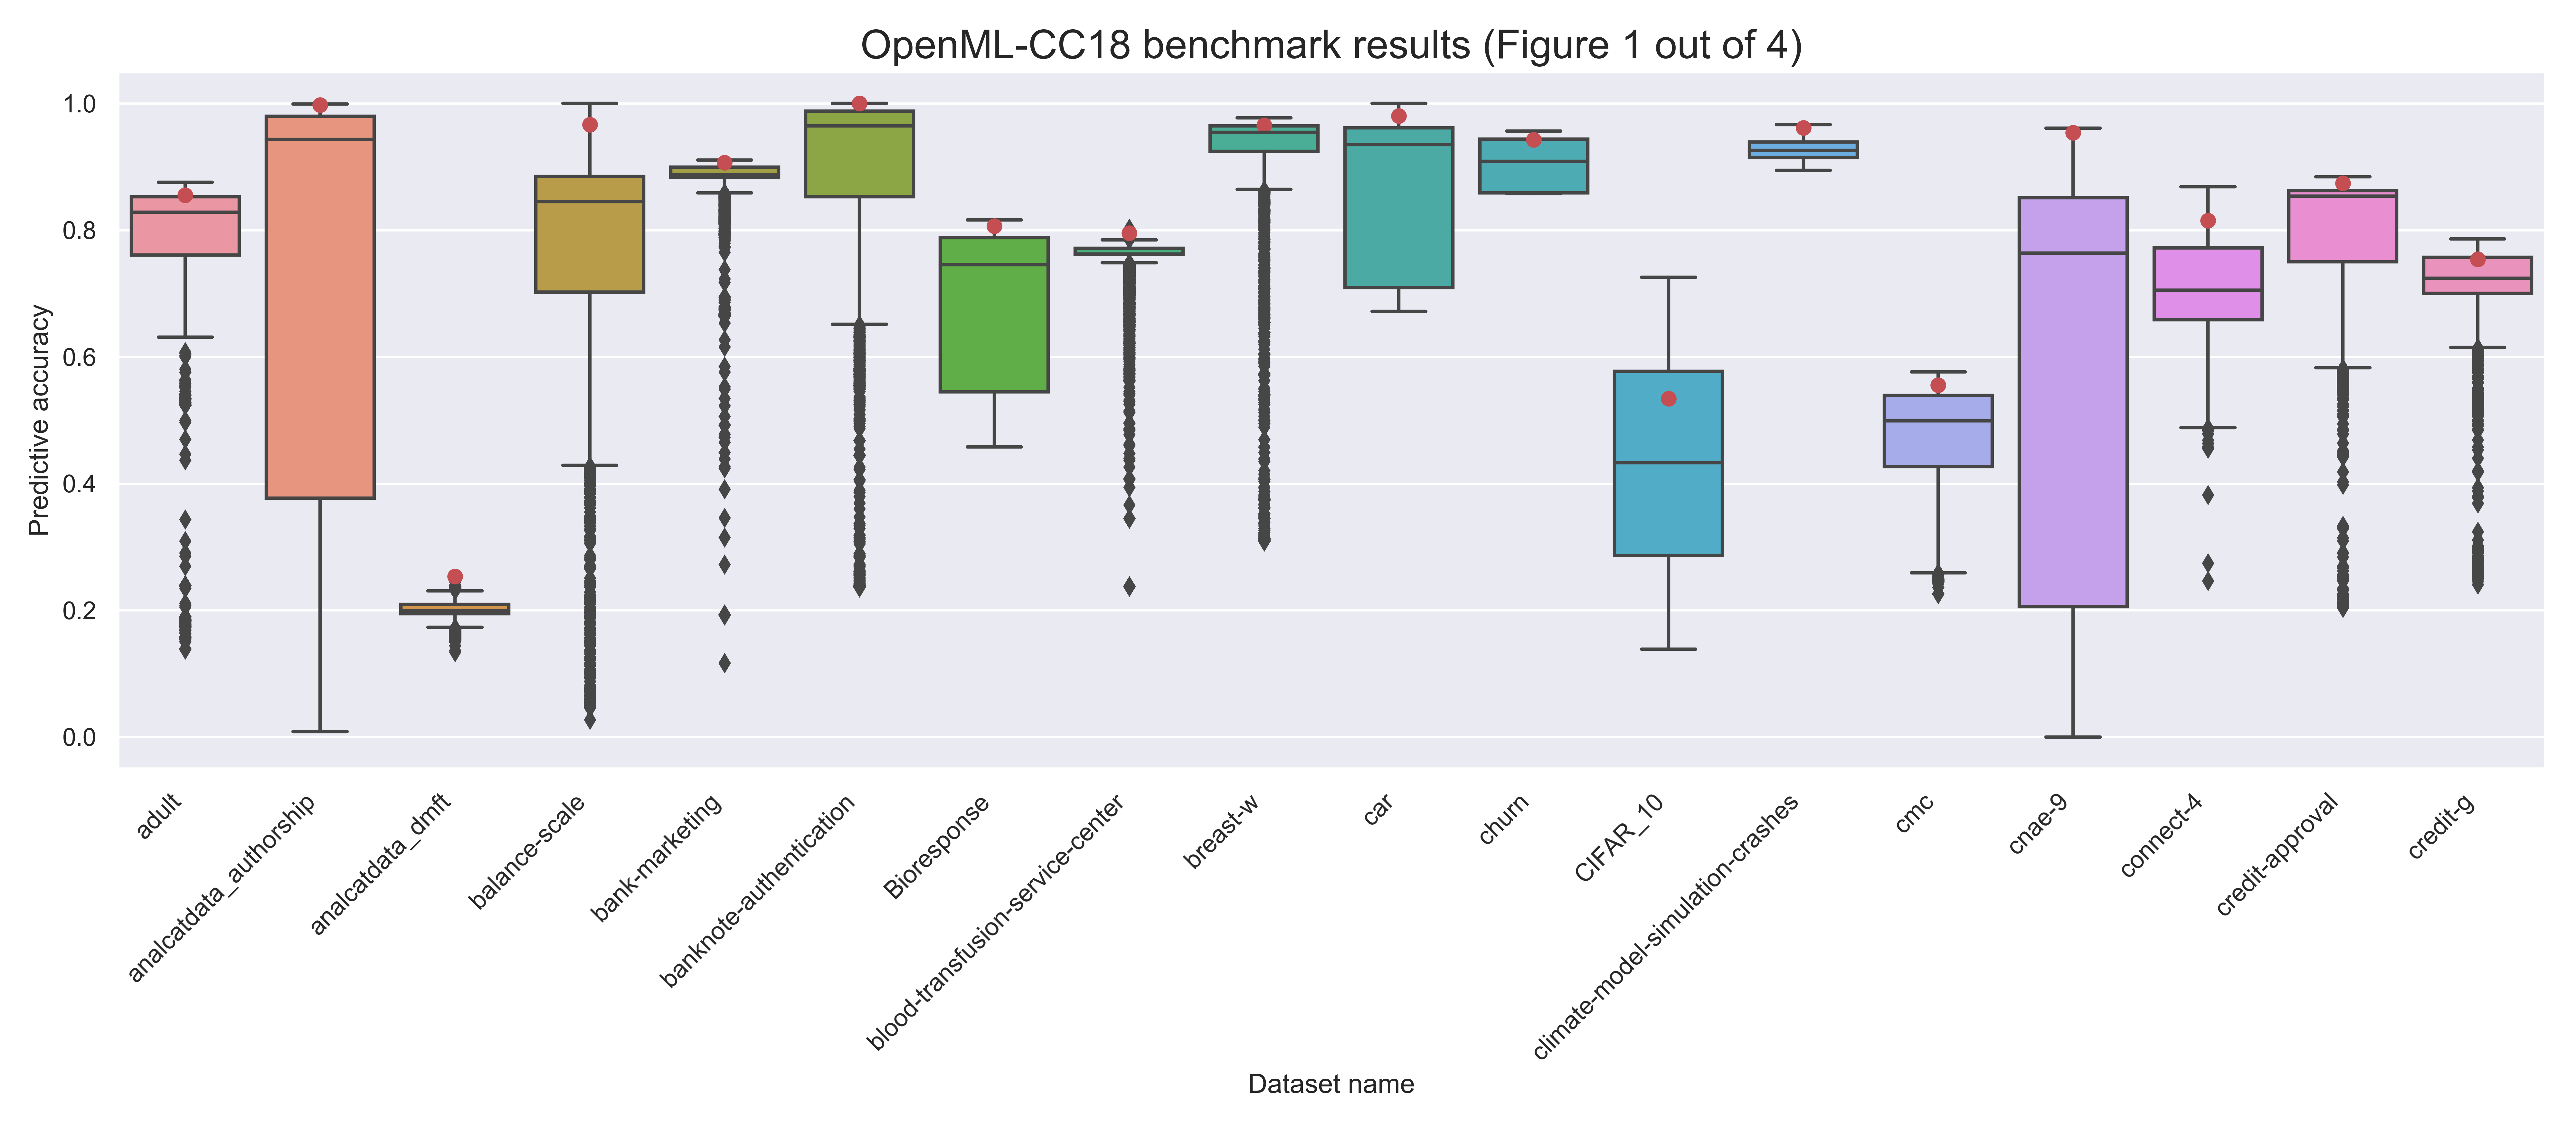
\includegraphics[width=0.8\linewidth]{../img/openml-boxplot0-hdpi.png}

\end{minipage}%
\begin{minipage}{.5\textwidth}
  \centering
  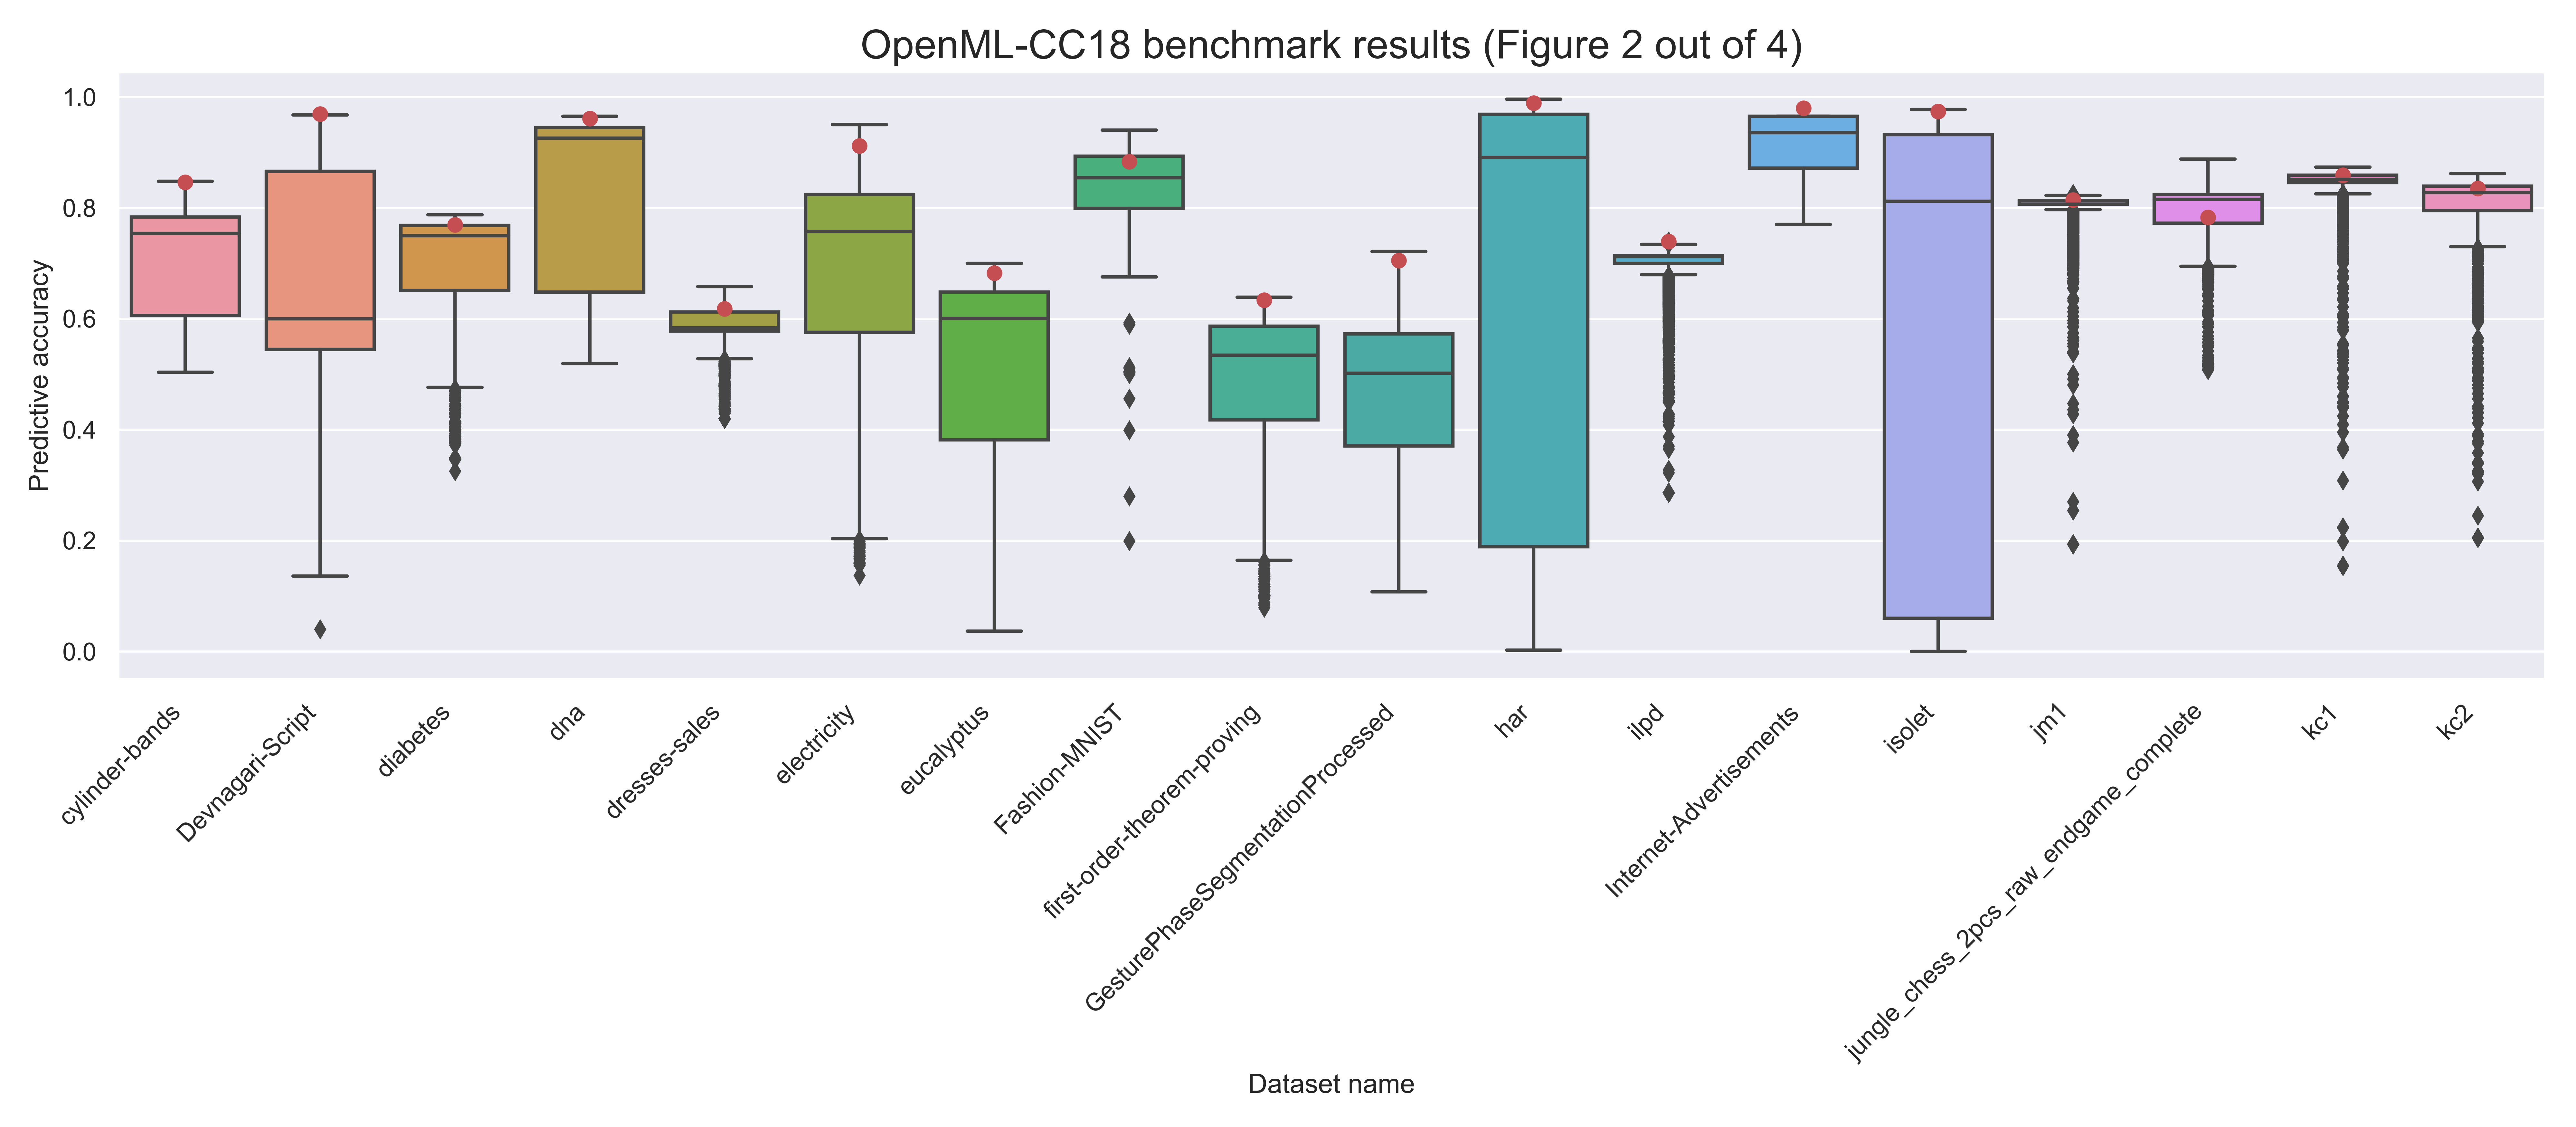
\includegraphics[width=0.8\linewidth]{../img/openml-boxplot1-hdpi.png}

\end{minipage}

\vspace{0.5em}

\begin{minipage}{.5\textwidth}
  \centering
  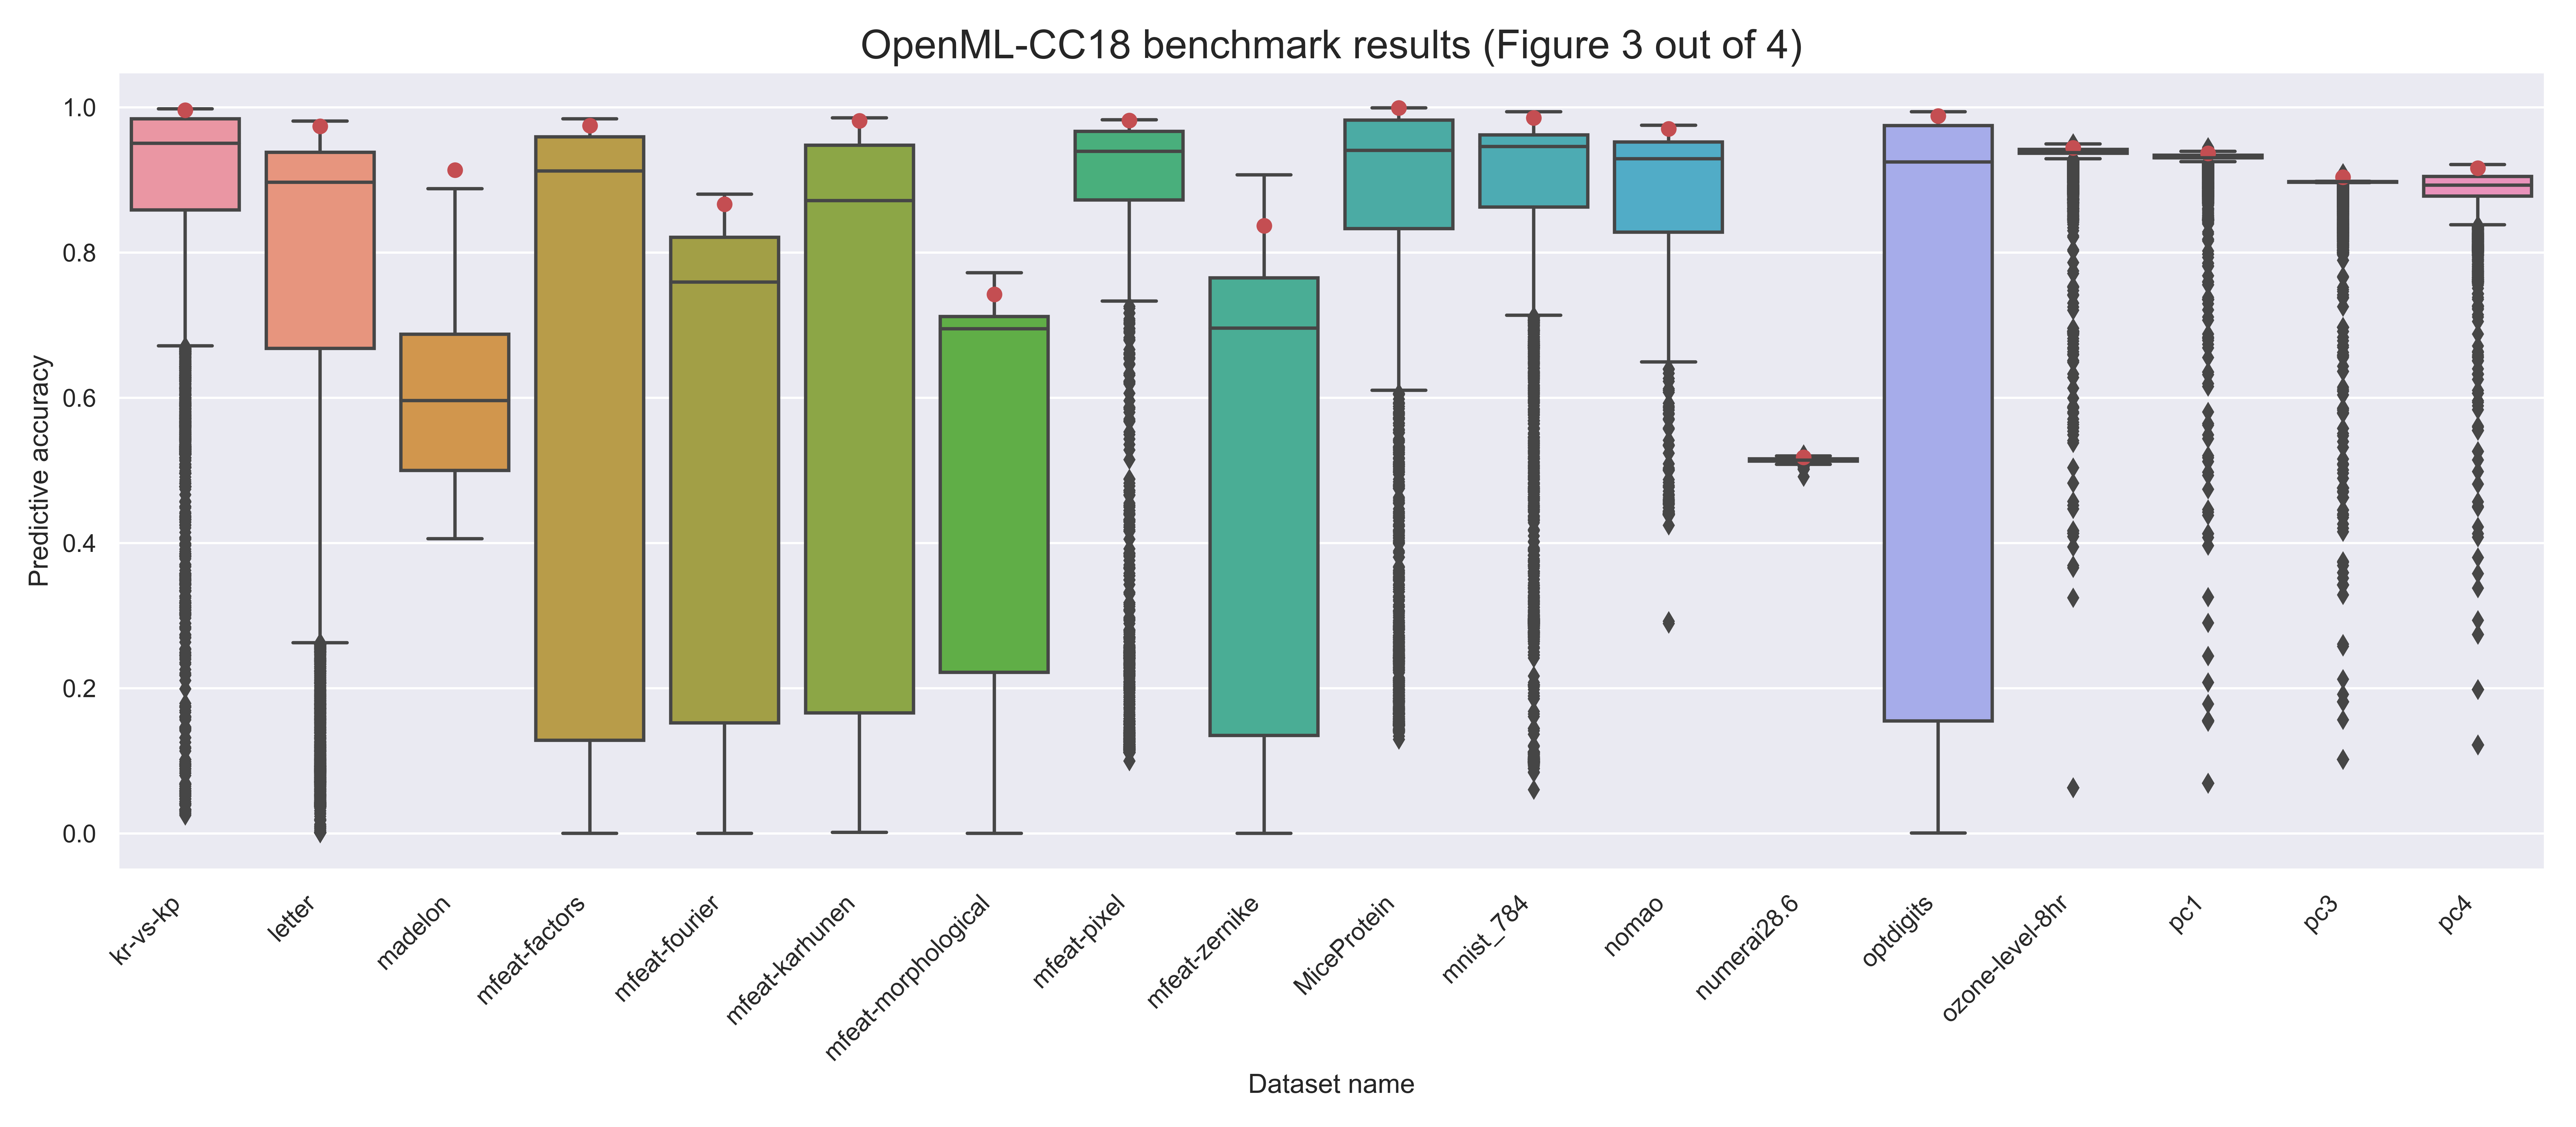
\includegraphics[width=0.8\linewidth]{../img/openml-boxplot2-hdpi.png}

\end{minipage}%
\begin{minipage}{.5\textwidth}
  \centering
  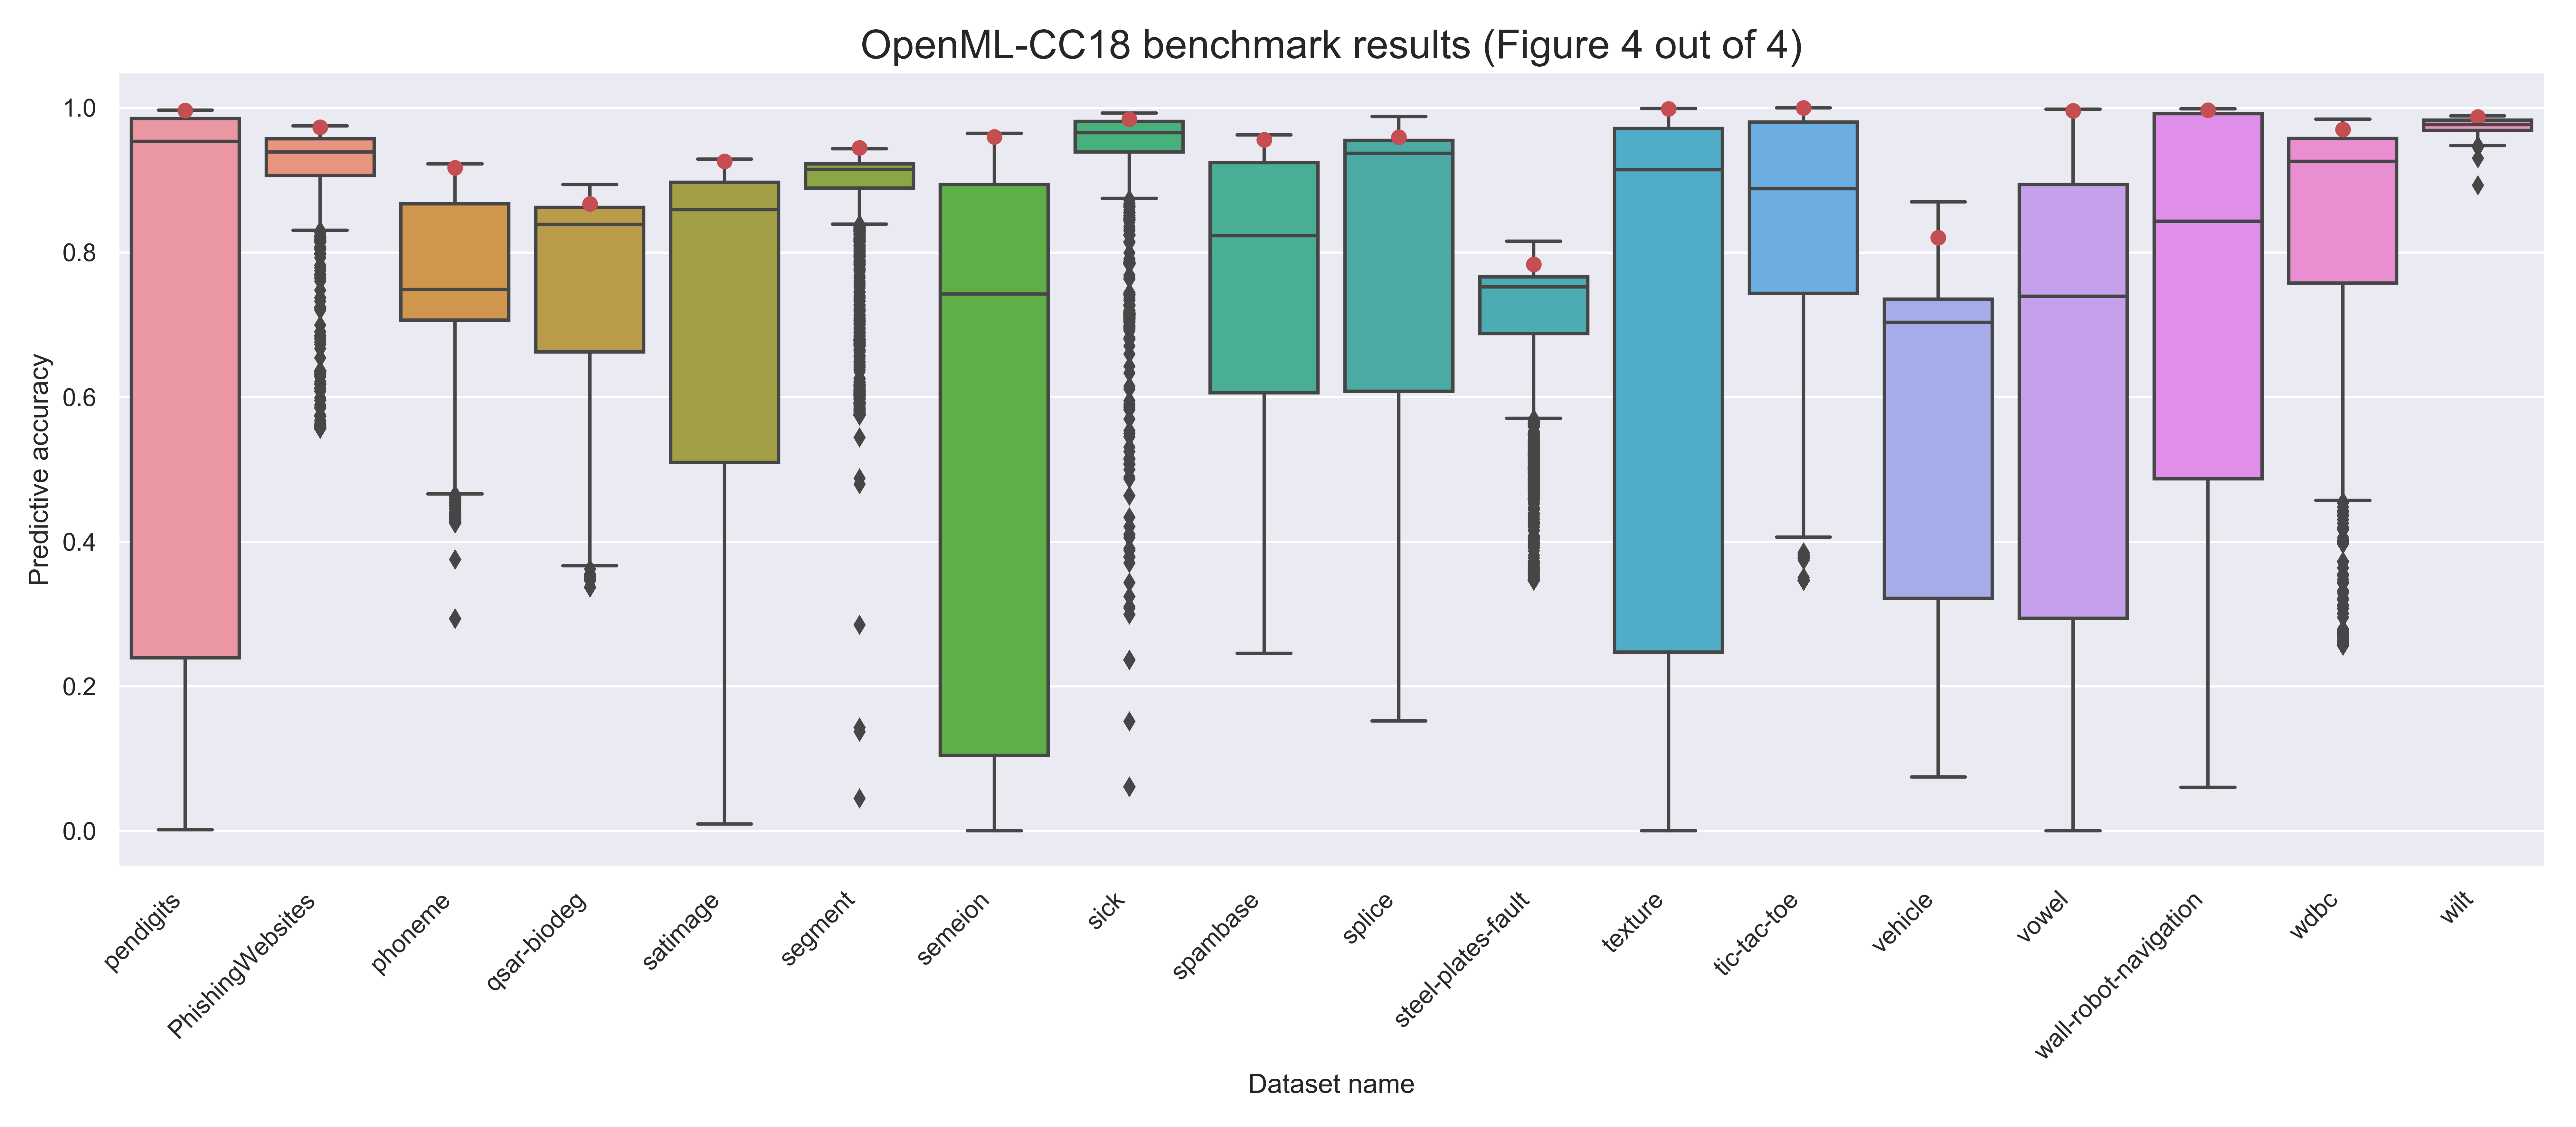
\includegraphics[width=0.8\linewidth]{../img/openml-boxplot3-hdpi.png}

\end{minipage}

\captionof{figure}{Results on OpenML-CC18 benchmark}
\label{fig:openml}
\end{minipage}
}

%%% Box 1 %%%%%%%%%%%%%%%%%%%%%%%%%%%%%%%%%%%%%%%%%%%%%%%%%%%%%%%%%%%%%%%%%%%%%
\headerbox{Workflows}{name=box1,column=0,below=abstract}{
\begin{minipage}{\textwidth}
  \centering
  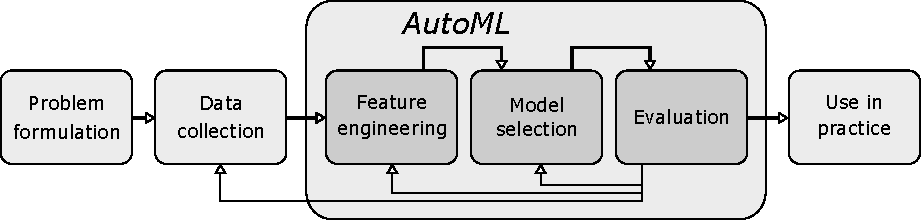
\includegraphics[width=0.7\linewidth]{../img/workflow-pdfa.pdf}
  \captionof{figure}{Schema of a general workflow}
  \label{fig:workflow}
  \vspace{0.5em}
\end{minipage}

A machine learning workflow is the process of solving a given machine learning
problem. As we can see in Figure \ref{fig:workflow}, a general workflow can be divided
into several steps. The first two steps are usually handled by an expert from an
unrelated field, who provides data to machine learning experts. Then, the data is
preprocessed and a suitable machine learning method needs to be chosen. This process is
usually iterative, as there are many different methods with several hyperparameters. To
obtain good results, it is necessary to carefully choose them, and so the procedure may be
very time consuming.

}

\headerbox{AutoML}{name=box3,column=0, below=box1,above=box4}{
The AutoML systems aim to automatize the process of selection of suitable feature
preprocessing methods and of a model with a particular hyperparameter setting. The idea
is that with these systems, machine learning may be accessible
even to non-experts, and on the other hand experts may use it for model
recommendation. 

\begin{minipage}{\textwidth}
  \centering
  \vspace{0.7em}
  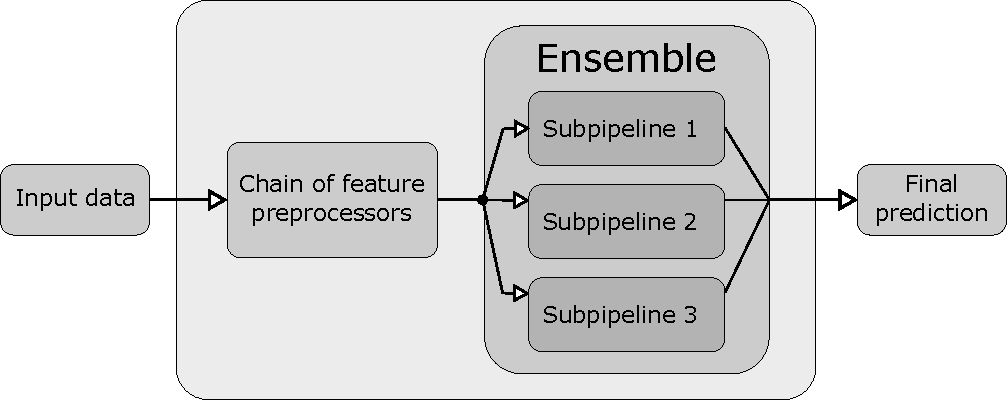
\includegraphics[width=0.65\linewidth]{../img/pipeline-pdfa.pdf}
  \captionof{figure}{A more complex machine learning pipeline}
  \label{fig:pipeline}  
  \vspace{0.7em}
\end{minipage}

One of the tasks targeted by AutoML systems is \emph{pipeline optimization}. A machine
learning pipeline is composed from a chain of feature preprocessing methods and one
estimator. The estimator can be a simple method or an ensemble that contains one or more
base-estimators. Because a base-estimator can be a pipeline as well, a general pipeline
is a directed acyclic graph.
}

\headerbox{Our system}{name=box5,column=1}{
Existing methods for pipeline optimization operated only on a limited structure. Some of
them focused only on hyperparameter optimization of simple models and they did not include
any ensembles or feature preprocessing methods. Others allowed an arbitrary-sized
preprocessor chain, however,k no ensembles with pipelines as base-estimators were supported.

Our systems aims to search for a pipeline that performs well on the given task. The
pipelines can be composed from both ensembles and feature preprocessing methods, but simple
methods are tried out as well.
}

%%% Box 2 %%%%%%%%%%%%%%%%%%%%%%%%%%%%%%%%%%%%%%%%%%%%%%%%%%%%%%%%%%%%%%%%%%%%%
\headerbox{Developmental GP}{name=box2,column=1,below=box5}{
For pipeline optimization, we used the genetic programming (GP), which is a subfield
of evolutionary algorithms. An individual in GP is in fact a computer program. Usually,
it is represented as an expression tree. The fitness of the tree is determined by
running the program, or also evaluating all functions and their arguments.

\vspace{0.5em}
\begin{minipage}{\textwidth}

  \begin{minipage}{.5\textwidth}
    \centering
    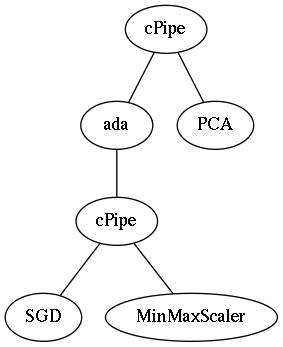
\includegraphics[width=0.45\linewidth]{../img/ada.png}

  \end{minipage}%
  \begin{minipage}{.5\textwidth}
    \centering
    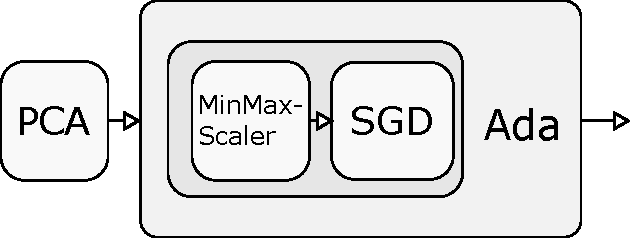
\includegraphics[width=0.8\linewidth]{../img/ada-pdfa.pdf}
  \end{minipage}
  
  \captionof{figure}{Example of an encoded pipeline}
  \label{fig:encoding}
\end{minipage}
\vspace{0.5em}

We created a specific encoding that enables to convert pipelines in the form of a DAG into
a tree representation. Instead of directly encoding pipeline steps as nodes, we apply the
developmental GP, where the nodes represent \emph{operations} that create the pipeline.
An example of the encoding is shown in Figure \ref{fig:encoding}. The tree individual
contains instructions which construct the actual pipeline:

\vspace{0.5em}
\textbf{cPipe} --- create a pipeline with a preprocessor chain and an estimator
\begin{compactitem}
  \item[-] \textbf{ada} --- insert an AdaBoost ensemble with a base-estimator
  \begin{compactitem}
    \item[-] \textbf{cPipe} --- create a pipeline with a preprocessor chain
    \begin{compactitem}
      \item[-] \textbf{SGD} --- insert a SGD classifier
      \item[-] \textbf{MinMaxScaler} --- insert a MinMaxScaler
    \end{compactitem}
  
  \end{compactitem}
  
  \item[-] \textbf{PCA} --- insert the PCA preprocessor
\end{compactitem}
}

\headerbox{OpenML experiment}{name=box2,column=1,below=box2,above=box4}{
Our system was tested on the OpenML-CC18 benchmark, which is a suite of 72 datasets
available at OpenML. Each of the datasets is associated with a classification task,
the evaluation method is 10-fold cross-validation.
A comparison of our results with all other results uploaded to OpenML are shown in Figure
\ref{fig:openml}. On most of the datasets our system performed in the upper quartile of
all results.
}

\end{poster}

\end{document}